\section{I/O Automata Programming Model\label{representation}}

In this section, we show how I/O automata can be used to construct real programs using ioa++.
To motivate the presentation, we use the classic problem of electing a leader in a unidirectional ring.
We first show how I/O automata are represented in the C++ language.
We then discuss the mechanisms available for dynamic composition.
We conclude with techniques for managing dynamic constellations of automata.

\subsection{I/O Automata Representation}

\paragraph{Leader election in a unidirectional ring.}
Nodes in a distributed system are arranged in a ring so that two consecutive nodes are connected by a directed channel.
The goal is to designate one of the nodes as the leader of the ring.
The solution we adopt is the asynchronous LCR algorithm presented by Lynch in Chapter 15 of~\cite{lynch1996distributed} which is in turn based on the work of LeLann~\cite{le1977distributed} and Chang and Roberts~\cite{chang1979improved}.
The LCR algorithm assumes that every node has a unique identifier (UID).
When the protocol begins, each node sends its UID to its successor.
When a node receives a UID from its predecessor that is greater than its own, it forwards the UID to its successor.
When a node receives its own UID, it elects itself the leader of the ring.
Our implementation of the asynchronous LCR automaton is located in \verb+examples/asynch_lcr_automaton.hpp+ of the ioa++ package.

\paragraph{Declaring an automaton.}
All automata inherit from the common base class \verb+ioa::automaton+ which implements the system action interface.
The following code declares the \verb+asynch_lcr_automaton+:
\begin{lstlisting}
template <typename UID>
class asynch_lcr_automaton :
  public ioa::automaton
{
  ...
};
\end{lstlisting}
The \verb+asynch_lcr_automaton+ is declared as a template where the \verb+UID+ template parameter must model the unique identifier concept.
The generic programming facilities of the C++ language aid in the development of general purpose reusable components.

\paragraph{Declaring and initializing state variables.}
The state variables of an automaton are expressed as member variables of the corresponding class.
The four state variables of the \verb+asynch_lcr_automaton+ include the UID of the automaton, a queue of outgoing messages, and flags for reporting a change in status:
\begin{lstlisting}
private:
  const UID m_u;
  std::queue<UID> m_send;
  bool m_report;
  bool m_leader;
\end{lstlisting}
Notice that the member variables are declared \verb+private+ which is in keeping with the notion that the state of each automaton is independent.
State variables are initialized using a constructor.
For the \verb+asynch_lcr_automaton+, the flags are both false and the UID is initialized and added to the send queue:
\begin{lstlisting}
public:
  asynch_lcr_automaton (const UID& u) :
    m_u (u),
    m_report (false),
    m_leader (false)
  {
    m_send.push (m_u);
    schedule ();
  }
\end{lstlisting}
The constructor also bootstraps the scheduler by scheduling all enabled local actions using the member function \verb+schedule+.
The \verb+schedule+ member function is discussed in the paragraph on scheduling.

\paragraph{Declaring/defining actions.}
Actions are member variables that model the action concept.
Actions contain methods for preconditions, effects, and scheduling and traits that indicate the actions's type (input, output, internal), value status, value type, parameter status, and parameter type.
The traits are used to guide the execution of the methods by the model and supply values and parameters as necessary.
The traits are also used to check that input actions are bound to output actions with the same value status and type.
Bindings are checked for type compatibility at compile time using the generic programming facilities of C++.

To facilitate declaring actions, a number of wrappers and macros corresponding to the action types listed in section~\ref{practical} are available.
Local actions are declared using three functions corresponding to a precondition, effect, and scheduling call.
The macros assume the functions are named \verb+action_name_precondition+, \verb+action_name_effect+, and \verb+action_name_schedule+.
For example, the send action of the \verb+asynch_lcr_automaton+ is declared:
\begin{lstlisting}
private:
  bool send_precondition () const { ... }
  UID send_effect () { ... }
  void send_schedule () const { ... }
public:
  V_UP_OUTPUT (asynch_lcr_automaton, send, UID);
\end{lstlisting}
Input actions are declared similarly save the absence of a precondition.
The precondition and scheduling functions are not allowed to change the state of the automaton and are consequently declared \verb+const+.
The macros for actions that are subject to binding by other automata belong in a \verb+public+ section.

\paragraph{Scheduling.}
Automata submit actions to the scheduler using the \verb+ioa::schedule+ function.
The \verb+ioa::schedule+ function can be called at any time.
However, automata are generally easier to read if scheduling calls are relegated to the scheduling functions.
A common pattern is to schedule all local actions using one member function where each action is guarded by its precondition as described in section~\ref{scheduling}.
For the \verb+asynch_lcr_automaton+, the scheduling function is:
\begin{lstlisting}
  void schedule () const {
    if (send_precondition ()) {
      ioa::schedule (&asynch_lcr_automaton::send);
    }
    if (leader_precondition ()) {
      ioa::schedule (&asynch_lcr_automaton::leader);
    }
  }
\end{lstlisting}
The various scheduling functions in the \verb+asynch_lcr_automaton+ and the constructor all dispatch to this function.

\subsection{Dynamic Composition}

\begin{figure}
\center
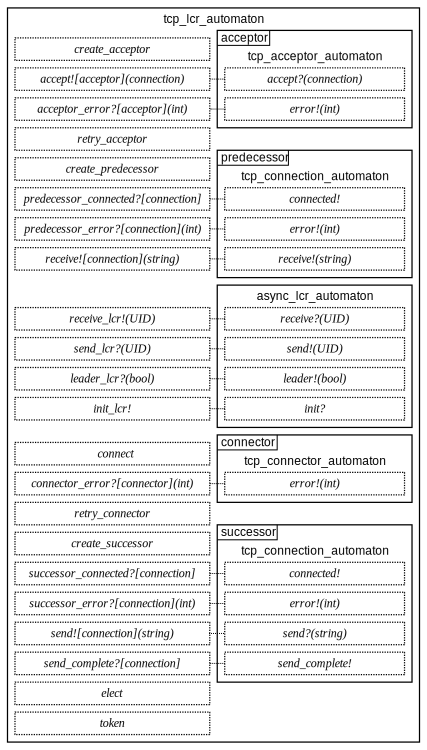
\includegraphics[width=\textwidth]{tcp_lcr_automaton}
\caption{TCP LCR automaton.}
\label{tcp_lcr_automaton}
\end{figure}

\paragraph{Leader election in a ring using TCP.}
The \verb+asynch_lcr_automaton+ is a reusable component designed to be used in the context of a larger system.
The \verb+tcp_lcr_automaton+ listed in \verb+examples/tcp_lcr.cpp+ elects a leader in a dynamic ring of processes connected by TCP sockets.
The structure of the \verb+tcp_lcr_automaton+ is given in Figure~\ref{tcp_lcr_automaton}.
The \verb+tcp_lcr_automaton+ is composed with a \verb+tcp_acceptor_automaton+ to accept a connection from its predecessor, a \verb+tcp_connector_automaton+ to create a connection to its successor, two \verb+tcp_connection_automaton+ representing the predecessor and successor, and a \verb+asynch_lcr_automaton+ to realize the leader election algorithm.
The leader of the ring periodically sends a token which is forwarded by all nodes in the ring.
If a node has not received a token for a specified duration of time, it calls for an election.

\paragraph{Binding predicates.}
Recall that automata require the ability to inspect the current set of bindings to adhere to the I/O automata model.
The binding predicate supplied by ioa++ is the \verb+ioa::binding_count+ function which returns the number of actions bound to the specified action.
The value returned by \verb+ioa::binding_count+ is zero for internal actions, zero or one for input actions, and non-negative for output actions.
Most often, \verb+ioa::binding_count+ is used in the precondition of outputs to ensure that the value generated by the output will be received.
This type of usage can be seen in the send action of the \verb+tcp_lcr_automaton+:
\begin{lstlisting}
  bool send_precondition (
    ioa::automaton_manager<ioa::tcp_connection_automaton>* s) const
  {
    return ... && ioa::binding_count (&tcp_lcr_automaton::send, s) != 0;
  }
\end{lstlisting}

\paragraph{Dynamic composition.}
Dynamic composition is accomplished by creating child automata and bindings via \verb+ioa::automaton_manager+ and \verb+ioa::binding_manager+ objects.
The \verb+tcp_lcr_automaton+ creates a \verb+asynch_lcr_automaton+ and binds to it with the following code:
\begin{lstlisting}
    ioa::automaton_manager<asynch_lcr_automaton<uuid> >* lcr =
       ioa::make_automaton_manager (this,
         ioa::make_generator<asynch_lcr_automaton<uuid> > (m_u));
    ioa::make_binding_manager (this,
			       lcr, &asynch_lcr_automaton<uuid>::send,
			       &m_self, &tcp_lcr_automaton::send_lcr);
    ioa::make_binding_manager (this,
			       &m_self, &tcp_lcr_automaton::receive_lcr,
			       lcr, &asynch_lcr_automaton<uuid>::receive);
    ioa::make_binding_manager (this,
			       lcr, &asynch_lcr_automaton<uuid>::leader,
			       &m_self, &tcp_lcr_automaton::leader_lcr);
    ioa::make_binding_manager (this,
			       &m_self, &tcp_lcr_automaton::init_lcr,
			       lcr, &asynch_lcr_automaton<uuid>::init);
\end{lstlisting}
Children automata are managed by \verb+ioa::automaton_manager+ objects which can be created via the \verb+ioa::make_automaton_manager+ function.
An automaton manager object requires an \verb+ioa::automaton+ object for its system action implementation and a generator for allocating the child automaton.
Bindings are managed by \verb+ioa::binding_manager+ objects which can created via the \verb+ioa::make_binding_manager+ function.
A binding manager objects requires an \verb+ioa::automaton+ object for its system action implementation, a manager object for the output automaton, a reference to the output action, a manger object for the input automaton, a reference to the input action, and parameters for the actions if required.
The \verb+ioa::automaton_manager+ class and \verb+ioa::binding_manager+ class contain methods for destroying and unbinding respectively.
The \verb+m_self+ object of the example is a \verb+ioa::handle_manager+ which can be used to bind to automata that already exist.
From the example, the \verb+tcp_lcr_automaton+ binds the \verb+asynch_lcr_automaton+ to itself.
The wary reader might notice that the \verb+ioa::automaton_manager+ and \verb+ioa::binding_manager+s in the example are dynamically allocated but never recorded and thus never freed.
Both classes are managed by the \verb+ioa::automaton+ and automatically deallocated when the automaton or binding they manange is destroyed or unbound respectively.

\subsection{Managing Dynamic Constellations}

In this section, we introduce techniques and principles for managing dynamic constellations of automata and bindings that go beyond the ``nuts and bolts'' presented in the previous section.
This list is neither exhaustive nor authoritative but rather a distillation of our experiences working with I/O automata.

\paragraph{Dynamics in the TCP LCR automaton.}
A \verb+tcp_lcr_automaton+ continuously attempts to complete the ring by accepting a connection from its predecessor or connecting to its successor.
Accepting can fail if the socket used for listening is currently unavailable.
Connecting can fail if the successor automaton does not exist and is therefore not listening for incoming connections.
The connections themselves will fail when nodes leave the ring.
The \verb+tcp_lcr_automaton+ also contains constraints on the order in which automata are created with respect to each other and with respect to which actions are executed.
For example, the predecessor connection must be created before it is passed to the acceptor via the accept action.
Similarly, the successor connection must be created before it is passed via a constructor to the connector.

\paragraph{System action events.}
Determining the outcome of a system action event, e.g., that a child automaton was created, is necessary when there are constraints on the order in which system actions must occur.
For example, the Binding Manager mentioned in section~\ref{system_action_section} waits until the automata supply the output action and input action are created before attempting to bind.
User automata can observe \verb+ioa::automaton_manager+ objects and \verb+ioa::binding_manager+ objects to receive events generated upon the completion of a system action.

\paragraph{Error reporting.}
The event semantics of I/O automata provide a natural mechanism for reporting errors.
An automaton that encounters an error can use an output action to signal the error.
The automaton can continue processing if the error is transient or stop if the error is permanent.
In either case, the error is propagated to the automaton that is using the automaton that encountered an error.
Using this technique, errors can be propagated up the hierarchy and resolved at an appropriate level.
The two strategies for handling an error are to either reset or replace the portion of the constellation that encountered the error.

\paragraph{Handling errors by resetting.}
An automaton that can be reset has one or more output actions for reporting errors and one or more input actions for resetting.
Errors need not be viewed as exceptional circumstances but a necessary part of the protocol implemented by the automaton.
Automaton designers should strive to write automata that are capable of being reset as this is the simplest error handling strategy.

\paragraph{Handling errors by replacing.}
The non-deterministic and asynchronous nature of system actions complicates replacing an automaton.
To replace a child automaton, the parent automaton must destroy the child, create a new child, and bind to the new child.
For reasons already discussed, the bind must occur after the create.
This constraint is enforced by the \verb+ioa::binding_manager+ class.
Additionally, the destroy must occur before the first bind to ensure that all bindings associated with the first child have been dissolved.
Attempts to bind before the destroy will fail because either the output action or the input action will be unavailable, i.e., still bound to the first child.
A general solution is to observe the automaton and wait for it to be destroyed.

If all of the bindings of a child automaton are with its parent, then the child can be replaced using parameters.
The parent automaton associates a parameter, typically the child automaton, with all bindings to the child automaton.
When the child needs to be replaced, a new child is created and the current parameter is updated to reflect this change.
The old bindings can be disabled by checking their parameter against the new parameter.
When using replacement with parameters, there is no need to wait for the child automaton to be destroyed since the parameter causes all bindings to be different.

%% Conclude with our recommendations for programming, highlight need for exploration.

%% Tips for Writing Programs with I/O Automata
%% 1. Make sure that a parameter exists.
%% 2. Move logic in observe to local actions.
%% 3. Avoid observing an arbitrary number of managers.
%% 4. Do not bind to managers allocated on the stack.
%% 5. Stop when an error is encoutered and report it.
%% 6. Make sure output actions are bound.
%% 7. Make sure local actions are scheduled.
%% 8. Do not pass pointers---use const_shared_ptr.
%% 9. Check preconditions.
%% 10. Check effects.
%% 11. Order clauses of preconditions for efficiency.
%% 12. Automata that should be destroyed at the same time should be created at the same time and vice versa.  (Group using a parent.)

%% \begin{outline}
%% \item State
%%   \begin{outline}
%%   \item There is no shared state in a 
%%   \item Local state only
%%   \item Shared state
%%     \begin{outline}
%%       \item Impossible in distributed systems
%%       \item Dangerous in local systems
%%     \end{outline}
%%   \end{outline}
%% \item Communication
%%   \begin{outline}
%%   \item Atomic asynchronous message passing
%%   \item Network sets size of atom (UDP)
%%   \item Can build reliable streams (TCP)
%%   \item Local equivalent is passing a value
%%   \item Model should lend itself to writing protocols
%%   \end{outline}
%% \item Asynchrony
%%   \begin{outline}
%%     \item Model must have natural support for asynchrony, i.e., event-based
%%     \item Leads to a more efficient implementation because changed state and enabled actions become obvious
%%   \end{outline}
%% \item Concurrency
%%   \begin{outline}
%%     \item Reason about systems using non-deterministic interleaving of atomic actions
%%     \item Model should admit implementations that execute concurrently
%%   \end{outline}
%% \item Dynamics
%%   \begin{outline}
%%     \item Configuration - Edges in graph of communicating components can change at run-time.
%%       \begin{outline}
%%       \item Already required in distributed settings
%%       \item Not addressed in formal models
%%       \end{outline}
%%     \item Extension - Nodes in graph of communicating components can change at run-time.
%%   \end{outline}
%%   \item Reflection
%% \end{outline}

%% I/O Automata
%% \begin{itemize}
%%   \item Compare with UNITY
%%   \item Compare with esterel
%%   \item Compare with pi calculus
%%   \item Compare with Ptolemy
%% \end{itemize}
